\documentclass[tikz]{standalone}
\usepackage{bm}
\usepackage{pgfplots}
\pgfplotsset{compat=1.9}
\usetikzlibrary{arrows.meta}
\tikzset{>=Latex}

\begin{document}

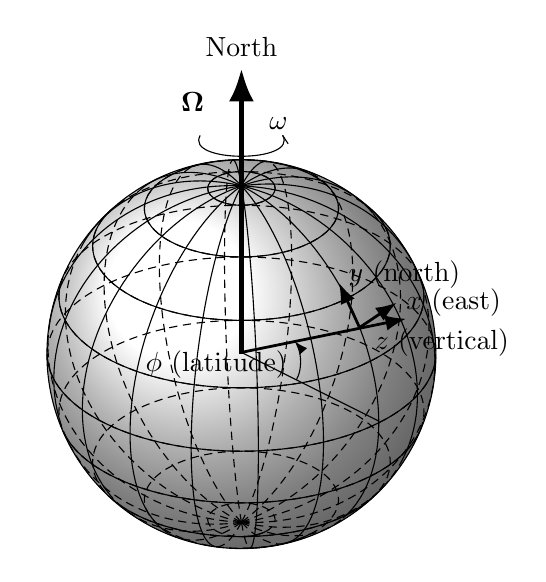
\begin{tikzpicture}
\def\tilt{45}
\def\azimuth{30}
\begin{axis}[%
axis equal,
width=14cm,
height=14cm,
hide axis,
enlargelimits=0.3,
view/h=\tilt,
view/v=\azimuth,
scale uniformly strategy=units only,
colormap={bluewhite}{color=(blue) color=(white)},
]
\coordinate (X) at (axis cs: 1,0,0);
\coordinate (-X) at (axis cs: -1,0,0);
\coordinate (Y) at (axis cs: 0,1,0);
\coordinate (-Y) at (axis cs: 0,-1,0);
\coordinate (Z) at (axis cs: 0,0,1);
\coordinate (-Z) at (axis cs: 0,0,-1);
\filldraw[ball color=white] (axis cs: 0,0,0) circle (2.47cm);
    \pgfplotsinvokeforeach {-80,-60,...,80}{
        \pgfplotsextra{
            \pgfmathsetmacro\sinVis{sin(#1)/cos(#1)*sin(\azimuth)/cos(\azimuth)}
            % angle of "visibility"
            \pgfmathsetmacro\angVis{asin(min(1,max(\sinVis,-1)))}
            \coordinate (X) at (axis cs: {cos(#1)},0,{sin(#1)});
            \draw [densely dashed] (X) arc (0:360:{100*cos(#1)});
        } }
    \pgfplotsinvokeforeach {-80,-60,...,80}{
    \pgfplotsextra{
        \pgfmathsetmacro\sinVis{sin(#1)/cos(#1)*sin(\azimuth)/cos(\azimuth)}
         % angle of "visibility"
        \pgfmathsetmacro\angVis{asin(min(1,max(\sinVis,-1)))}
        \coordinate (X) at (axis cs: {cos(#1)},0,{sin(#1)});
        \draw (X) arc (0:\tilt+\angVis:{100*cos(#1)}) (X) arc (0:-180+\tilt-\angVis:{100*cos(#1)});
    } }

\draw [-{>[scale=1]},line width=2pt] (axis cs: 0,0,0) -- (axis cs: 0,0,1.7) node [above] {North};
\draw [-] (axis cs: -.15,-.15,1.3) to [bend right=120] (axis cs: .15,.15,1.3);
\draw [-] (axis cs: .15,.15,1.3) -- (axis cs: .17,.17,1.25);
\draw (axis cs: .10,.17,1.25) node [above] {$\omega$};
\draw (axis cs: -0.1,-0.1,1.5) node [left] {${\bm\Omega}$};

\foreach \a in {0,20,...,359}
{ \pgfmathsetmacro{\Bound}{-60*cos(\a+45)}
    \addplot3[domain=\Bound:90, samples=45,samples y=0] ({cos(\a)*cos(x)},{sin(\a)*cos(x)},{sin(x)});
    \addplot3[domain=-90:\Bound, samples=45,samples y=0, densely dashed] ({cos(\a)*cos(x)},{sin(\a)*cos(x)},{sin(x)});
}

% draw latitude angle
\draw [-] (axis cs: 0,0,0.01) -- (axis cs: 1.0,0,0.01);
\draw [-{>[scale=1]},line width=1pt] (axis cs: 0,0,0.01) -- (axis cs: 1.2,0.0,0.7);
\draw [-{>[scale=1]},line width=1pt] (axis cs: .80,0.06,0.46) -- (axis cs: 1.06,0.07,0.71);
\draw [-{>[scale=1]},line width=1pt] (axis cs: .80,0.06,0.46) -- (axis cs: 0.51,0.20,0.55);

\draw (axis cs: 1.10,-0.20,0.60) node [right] {$z$ (vertical)};
\draw (axis cs: 1.06,0.07,0.71) node [right] {$x$ (east)};
\draw (axis cs: 0.51,0.20,0.60) node [right] {$y$ (north)};

\draw [->] (axis cs: 0.4,0,0.01) arc [start angle=-50, end angle=60, x radius=.15cm, y radius=.30cm];
\draw (axis cs: 0.4,0,0.1) node [left] {$\phi$ (latitude)};

\end{axis}
\end{tikzpicture}

\end{document}